\chapter{Introduction}

\section{Introduction}
This chapter sets the scene for the rest of the report. It presents the context in which News Insight was designed, states the problem the platform addresses, lists the project's objectives, describes the work methodology followed by the team, and closes with an overview of the technology stack used to build the platform. The chapters that follow (Global Architecture through Final Conclusion) each expand on one layer of the system that is only introduced here.

\section{Project context}
Tunisia has a dense but fragmented online news landscape. Outlets such as \textit{La Presse}, \textit{Business News}, \textit{Kapitalis}, and \textit{Mosaïque FM} each publish independently, in French and, for some outlets, Arabic, with no shared index and no cross-outlet view of what is being reported. A reader who wants a broad picture of the day's news in Tunisia — what topics dominate, how sentiment shifts on a given subject, which region a story concerns — has to visit each site separately and build that picture manually.

News Insight is an academic MLOps project that turns this fragmented landscape into a queryable dataset. It continuously collects articles from multiple Tunisian sources, enriches them with natural language processing (embeddings, sentiment, topic modelling), exposes the result through an API and a web dashboard, and adds a generative-AI layer (summaries, topic labels, and a conversational "ask the news" assistant) on top. The project is carried out as an End-of-Semester Project in Data Science and AI, academic year 2025-2026, by a team of three students — Ahmed Klabi, Mariem Smadhi, and Hichem Sboui — under the supervision of Sawssen Jalel.

\section{Problem statement}
Beyond the lack of a single entry point, three concrete gaps motivate this project:

\begin{itemize}
    \item \textbf{No aggregation.} Tunisian news outlets are not indexed together anywhere; comparing coverage of the same event across sources requires manual cross-referencing.
    \item \textbf{No semantic access.} Existing outlet websites only offer keyword search on their own archive, if that; there is no way to search across sources by meaning (e.g. find every article about a topic regardless of the exact wording used) or to ask a natural-language question and get a sourced answer.
    \item \textbf{No structured signal.} Raw articles carry no machine-readable topic, sentiment, or geographic tag, so tracking how a subject is covered over time, or which regions are mentioned, cannot be done without reading every article by hand.
\end{itemize}

News Insight is built specifically to close these three gaps for the Tunisian news ecosystem, using an MLOps pipeline that keeps the data current rather than a one-off dataset.

\section{Objectives}
The project pursues four concrete, complementary objectives:

\begin{itemize}
    \item \textbf{O1 --- Automated collection.} Continuously ingest articles from several Tunisian news sources without manual intervention, using RSS feeds as the primary channel and a dedicated HTML scraper as a fallback for deeper crawling of a single source.
    \item \textbf{O2 --- NLP enrichment.} Turn raw article text into structured signal: multilingual sentence embeddings for semantic retrieval, sentiment classification, and unsupervised topic discovery (BERTopic) so articles can be grouped, compared, and filtered automatically.
    \item \textbf{O3 --- GenAI access.} Let a user interact with the corpus in natural language: on-demand article summaries, human-readable topic labels, and a retrieval-augmented "ask the news" chat assistant that answers questions with cited sources.
    \item \textbf{O4 --- Reproducible MLOps.} Wrap the pipeline in tooling that makes it observable and repeatable rather than a collection of ad hoc scripts: workflow orchestration, experiment tracking for the clustering model, and a containerized deployment that any team member can bring up with a single command.
\end{itemize}

A fifth, supporting objective ties the previous four together: expose all of the above through a web dashboard so the results are usable by someone who does not read code — this is the subject of Chapter 10.

\section{Work methodology}
The team followed an agile, iteration-driven process suited to a three-person academic team rather than a formal heavyweight methodology.

\subsection{Iterative tracks}
Rather than designing the whole system up front, the work was organized into successive tracks, each building on the previous one and each shipped as soon as it was usable end to end: a \emph{foundation} track (project scaffolding, database schema, Docker Compose stack), a \emph{data sources} track (the scraper base class, the RSS ingestion pipeline, source-specific quirks such as image and category extraction), an \emph{ML/MLOps} track (embeddings, sentiment, BERTopic clustering, Prefect orchestration, MLflow experiment tracking), and finally an \emph{application} track covering the GenAI features and the React frontend. This ordering is visible directly in the commit history: early commits scaffold scrapers and the database, middle commits add clustering and MLflow logging (e.g.\ \textit{feat(mlops): log clustering runs + register model to MLflow}), and later commits build the chat assistant, semantic search, and UI on top of the by-then-stable pipeline (e.g.\ \textit{feat(api): RAG chat over articles via pgvector}, \textit{feat(ui): ask-the-news chat, sentiment timeline, article TL;DR}).

\subsection{Version control workflow}
The team used GitHub flow: every change of substance is developed on a short-lived feature branch, opened as a pull request against \texttt{main}, and merged once it is buildable. The repository (\texttt{github.com/\allowbreak ahmedkltn/\allowbreak news-mlops}) shows this pattern consistently across its history. Branches are named by intent, for example:

\begin{itemize}
    \item \texttt{feat/\allowbreak news-hub}, \texttt{feat/\allowbreak tunisia-region-map}, \texttt{feat/\allowbreak ai-search-themes-diversity} — new features;
    \item \texttt{fix/\allowbreak ai-search-precision}, \texttt{fix/\allowbreak summary-thin-content}, \texttt{fix/\allowbreak map-projection-and-search} — bug fixes.
\end{itemize}

These branches were merged as pull requests \#1 through \#11 at the time of writing. Commit messages follow the Conventional Commits convention (\texttt{feat}, \texttt{fix}, \texttt{chore}, \texttt{docs}, \texttt{test}, \texttt{perf}, \texttt{ci} prefixes), which keeps the history readable and made it straightforward to reconstruct the project timeline for this report. A continuous integration gate (\textit{ci: run pytest + frontend build on push}) runs the backend test suite and builds the frontend on every push, catching regressions before a branch is merged. Several pull requests in the log are targeted bug fixes discovered through use of the running system rather than planned features — for instance \texttt{fix/\allowbreak region-panel-scroll} (a scrollable list overflowing the page) and \texttt{fix/\allowbreak spa-cache-headers} (a stale single-page-app bundle being served from cache) — which reflects the iterative, test-and-fix rhythm of the later part of the project.

\section{Technology stack overview}
News Insight is built as a small, coherent set of open-source tools, one per concern in the pipeline: collection, storage, machine learning, orchestration and tracking, and the application layer. Figure~\ref{fig:tech-stack} shows the logo of each component; Table~\ref{tab:tech-stack} summarizes the role each one plays. Later chapters revisit each of these choices in the context of the layer they belong to.

\begin{figure}[H]
\centering
\begin{tabular}{ccccc}

\includegraphics[width=0.15\columnwidth]{img/python.png} &
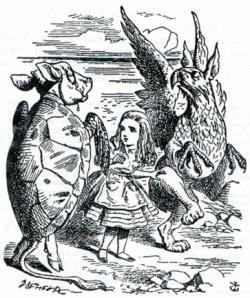
\includegraphics[width=0.15\columnwidth]{img/beautifulsoup.png} &

\includegraphics[width=0.15\columnwidth]{img/postgresql.png} &

\includegraphics[width=0.15\columnwidth]{img/huggingface.png} &

\includegraphics[width=0.15\columnwidth]{img/prefect.png} \\
\small Python & \small BeautifulSoup & \small PostgreSQL + pgvector & \small Hugging Face & \small Prefect \\[1.2em]

\includegraphics[width=0.15\columnwidth]{img/mlflow.png} &

\includegraphics[width=0.15\columnwidth]{img/fastapi.png} &

\includegraphics[width=0.15\columnwidth]{img/react.png} &

\includegraphics[width=0.15\columnwidth]{img/vite.png} &

\includegraphics[width=0.15\columnwidth]{img/docker.png} \\
\small MLflow & \small FastAPI & \small React & \small Vite & \small Docker \\
\end{tabular}
\caption{Technology stack of the News Insight platform, grouped by pipeline stage: collection, storage, machine learning, orchestration/tracking, and application.}
\label{fig:tech-stack}
\end{figure}

\begin{table}[H]
\centering
\begin{tabular}{|>{\raggedright\arraybackslash}p{2.6cm}|p{4.9cm}|p{7.4cm}|}
\hline
\textbf{Layer} & \textbf{Technology} & \textbf{Role} \\
\hline
Collection & Python, BeautifulSoup & RSS parsing and HTML scraping of Tunisian news sources \\
\hline
Storage & PostgreSQL, pgvector & Relational storage of articles plus vector similarity search on their embeddings \\
\hline
Machine learning & Hugging Face (sentence-transformers, BERTopic, cardiffnlp models) & Multilingual embeddings, sentiment classification, unsupervised topic modelling \\
\hline
Orchestration & Prefect & Scheduling and running the scrape / transform / cluster pipeline \\
\hline
Experiment tracking & MLflow & Logging clustering runs and pipeline metrics for monitoring \\
\hline
API & FastAPI & Exposing articles, search, and GenAI endpoints to the frontend \\
\hline
Frontend & React, Vite & Web dashboard for browsing, searching, and chatting with the news corpus \\
\hline
Infrastructure & Docker, Docker Compose & Containerized, single-command deployment of the whole stack \\
\hline
\end{tabular}
\caption{Role of each technology in the News Insight stack.}
\label{tab:tech-stack}
\end{table}

The GenAI layer (article summaries, topic labels, the "ask the news" chat assistant) is deliberately not tied to a single vendor: it goes through an OpenAI-compatible abstraction so the underlying large language model provider can be swapped by configuration, with a free-tier provider used by default. Chapter 6 details this design choice.

\section{Conclusion}
This chapter framed the "why" of News Insight: a fragmented Tunisian news landscape with no unified analytical view, addressed through four objectives — automated collection, NLP enrichment, GenAI access, and reproducible MLOps — pursued through an iterative, GitHub-flow-based process. The remainder of the report follows the pipeline these objectives describe, starting with the global architecture that ties the stack introduced in this chapter into a single system.
